\documentclass[aip,jmp,preprint]{revtex4-2}

\usepackage{amsmath,amssymb,mathtools}
\usepackage{bm}
\usepackage{tikz}
\usetikzlibrary{arrows.meta,positioning}

\newcommand{\M}{\mathsf{M}}
\newcommand{\K}{\mathcal{K}}
\newcommand{\ran}{\operatorname{ran}}
\newcommand{\tr}{\operatorname{Tr}}
\newcommand{\id}{\mathsf{I}}
\newcommand{\opnorm}[1]{\left\lVert #1\right\rVert_{\mathrm{op}}}

\begin{document}

\title{An exact criterion for removing an elementary amplitude-damping factor from a quantum channel}

\author{Xiaojian Zeng}
\email{xiaojianzeng@foxmail.com}
\affiliation{PBC School of Finance, Tsinghua University, Beijing 100190, China}

\date{September 14, 2026}

\begin{abstract}
Deciding whether a quantum channel contains a prescribed elementary noise factor is generally a constrained complete-positivity problem.  For the elementary amplitude-damping channel associated with two orthogonal states, we give a finite-dimensional necessary-and-sufficient criterion and the full admissible strength interval.  The published necessary condition says that right multiplication of every minimal Kraus operator by the transition matrix must remain in the minimal Kraus subspace.  We show that this condition is already sufficient.  In a minimal Kraus synthesis, the induced action is represented by a matrix whose largest singular value fixes the sharp complete-positivity threshold.  The proof follows from an exact congruence of Choi matrices and a support-invariance argument; it involves no perturbative expansion or numerical limit.  As an application, the result resolves the corresponding question for all phase-covariant qutrit channels of Choi ranks two through eight and all ordered pairs of distinct energy levels.  The factorization is static and does not by itself imply Markovianity or complete-positive divisibility of a time-indexed evolution.
\end{abstract}

\maketitle

\section{Introduction}

Factorization properties of completely positive trace-preserving (CPTP) maps distinguish indivisible channels from maps that can be assembled from simpler noise processes.  They also organize several notions of channel divisibility and their relation to continuous dynamics \cite{WolfCirac2008,DavalosZiman2023}.  A particularly concrete version of the problem fixes the right factor in advance and asks whether the remaining left quotient is again a channel.

Vom Ende recently introduced an elementary channel determined by a pair of states and a strength parameter, and studied complete positivity of its unique right quotient \cite{vomEnde2025}.  For orthogonal states, Proposition~1 of Ref.~\onlinecite{vomEnde2025} gives a necessary condition in terms of the minimal Kraus subspace.  Theorem~1 there proves sufficiency after imposing a second orthogonality condition.  The conclusion leaves open a necessary-and-sufficient characterization and points to covariant channels as a structured test class.

Here we prove that the published necessary condition alone is sufficient for orthogonal states in every finite dimension.  More precisely, it is support invariance under a simple nilpotent operator on Choi space.  Once this invariance is expressed in a minimal Kraus synthesis, positivity of the quotient is equivalent to positivity of a matrix of Kraus-rank size.  Its largest singular value gives the exact endpoint.  This both settles the phase-covariant qutrit question and supplies a dimension-independent diagnostic for the maximum strength of the elementary factor that can be removed.

The central chain of equivalences is summarized in Fig.~\ref{fig:flow}.  We first fix conventions and state the result, then prove the Choi congruence and support equivalence, and finally discuss the qutrit application, a sharp example, and exact symbolic checks.

\begin{figure}[tb]
  \centering
  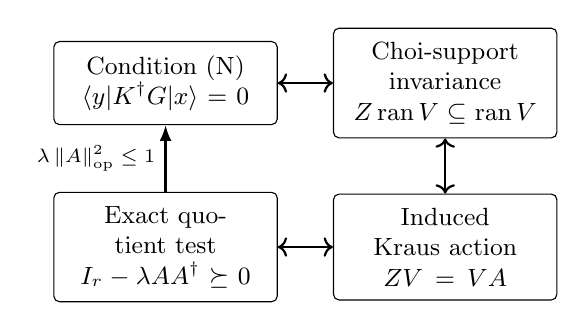
\begin{tikzpicture}[
  node distance=7mm and 7mm,
  box/.style={draw,rounded corners=2pt,align=center,inner sep=5pt,
              text width=0.205\textwidth,font=\small},
  arrow/.style={-{Latex[length=2mm]},thick}
]
  \node[box] (n) {Condition (N)\\$\langle y|K^\dagger G|x\rangle=0$};
  \node[box,right=of n] (s) {Choi-support invariance\\$Z\ran V\subseteq\ran V$};
  \node[box,below=of s] (a) {Induced Kraus action\\$ZV=VA$};
  \node[box,left=of a] (p) {Exact quotient test\\$I_r-\lambda AA^\dagger\succeq0$};
  \draw[<->,thick] (n) -- (s);
  \draw[<->,thick] (s) -- (a);
  \draw[<->,thick] (a) -- (p);
  \draw[arrow] (p) -- node[left,font=\scriptsize,align=center] {$\lambda\opnorm{A}^2\leq1$} (n);
\end{tikzpicture}

  \caption{Logical reduction of the fixed-right-factor problem.  The first two equivalences are purely geometric; the last uses the exact Choi congruence.  Here $V$ is a full-column-rank minimal Kraus synthesis and $ZV=VA$.  Alt text: four boxes connect condition (N), invariance of the Choi support, the induced matrix $A$, and the spectral positivity test.}
  \label{fig:flow}
\end{figure}

\section{Setup and main result}

Let $\Phi:\M_n\to\M_n$ be a CPTP map.  We use the unnormalized input-first Choi matrix and column vectorization
\begin{align}
 C(\Phi)&=\sum_{j,k=1}^{n}|j\rangle\langle k|\otimes
 \Phi(|j\rangle\langle k|), \label{eq:choi}\
 \operatorname{vec}(X)&=\sum_{j=1}^{n}|j\rangle\otimes X|j\rangle .
\end{align}
Thus $\Phi$ is completely positive if and only if $C(\Phi)\succeq0$, and it is trace preserving if and only if $\tr_{\mathrm{out}}C(\Phi)=I_n$ \cite{Choi1975}.

Choose orthogonal unit vectors $x,y\in\mathbb C^n$.  For $0\leq\lambda\leq1$, define
\begin{align}
 K_\lambda&=I_n-(1-\sqrt{1-\lambda})|x\rangle\langle x|,\nonumber\\
 L_\lambda&=\sqrt\lambda\,|y\rangle\langle x|,\label{eq:elementary-kraus}\\
 \Psi_\lambda(X)&=K_\lambda X K_\lambda^\dagger+L_\lambda X L_\lambda^\dagger .
\end{align}
This map is CPTP.  It is invertible as a linear map exactly on the domain used below, $0\leq\lambda<1$ \cite{vomEnde2025}.

Let $K_1,\ldots,K_r$ be a linearly independent minimal Kraus family of $\Phi$, and write
\begin{equation}
 \K_\Phi=\operatorname{span}\{K_1,\ldots,K_r\}\subset\M_n.
\end{equation}
The condition of interest is
\begin{equation}
 \langle y|K^\dagger G|x\rangle=0
 \quad\text{for all }K\in\K_\Phi,
 \ G\in\K_\Phi^\perp . \tag{N}\label{eq:N}
\end{equation}
It is independent of the chosen minimal Kraus representation and of any basis of the Hilbert--Schmidt orthogonal complement.

Define the $n^2\times r$ synthesis matrix $V$ and the Choi-space operator $Z$ by
\begin{equation}
 Ve_j=\operatorname{vec}(K_j),\qquad
 Z=(|y\rangle\langle x|)^T\otimes I_n . \label{eq:VZ}
\end{equation}
Then $C(\Phi)=VV^\dagger$ and $V$ has full column rank.

\paragraph*{Theorem 1.}
For a finite-dimensional CPTP map $\Phi$ and orthogonal unit vectors $x,y$, condition~\eqref{eq:N} holds if and only if there is a $\lambda\in(0,1)$ for which the unique quotient $\Theta_\lambda=\Phi\circ\Psi_\lambda^{-1}$ is CPTP.  When condition~\eqref{eq:N} holds, there is a unique $A\in\M_r$ such that
\begin{equation}
 ZV=VA, \label{eq:Adef}
\end{equation}
and, for every $0\leq\lambda<1$,
\begin{equation}
 \Theta_\lambda\text{ is CPTP}
 \quad\Longleftrightarrow\quad
 \lambda\,\opnorm{A}^{2}\leq1 . \label{eq:interval}
\end{equation}
The norm in Eq.~\eqref{eq:interval} is the largest-singular-value (spectral/operator) norm.  Hence the admissible set is
\begin{equation}
 [0,1)\cap[0,\opnorm{A}^{-2}], \label{eq:physical-interval}
\end{equation}
with physical supremum $\min\{1,\opnorm{A}^{-2}\}$.  The value $\lambda=1$ is never included because $\Psi_1$ is not invertible.

\section{Exact Choi congruence}

Put $t=\sqrt{1-\lambda}$ and
\begin{equation}
 D_\lambda=(K_\lambda^{-1})^T\otimes I_n
 =I_{n^2}+(t^{-1}-1)ZZ^\dagger . \label{eq:D}
\end{equation}
Orthogonality of $x$ and $y$ implies $D_\lambda Z=t^{-1}Z$.  Solving the elementary channel for its input gives
\begin{equation}
 \Psi_\lambda^{-1}(Y)=K_\lambda^{-1}Y(K_\lambda^{-1})^\dagger
 -\frac{1}{1-\lambda}L_\lambda YL_\lambda^\dagger . \label{eq:inverse}
\end{equation}
The corresponding Choi formula is Eq.~(3) of Ref.~\onlinecite{vomEnde2025}.  Using $L_\lambda^T\otimes I_n=\sqrt\lambda Z$ and $D_\lambda Z=t^{-1}Z$ reorganizes that formula into the exact congruence
\begin{equation}
 C(\Phi\circ\Psi_\lambda^{-1})
 =D_\lambda\bigl[C(\Phi)-\lambda ZC(\Phi)Z^\dagger\bigr]D_\lambda^\dagger . \label{eq:congruence}
\end{equation}
Because $D_\lambda$ is invertible for $\lambda<1$,
\begin{equation}
 C(\Phi\circ\Psi_\lambda^{-1})\succeq0
 \quad\Longleftrightarrow\quad
 C(\Phi)-\lambda ZC(\Phi)Z^\dagger\succeq0 . \label{eq:reduced-positivity}
\end{equation}
No small-$\lambda$ approximation enters this reduction.

\section{Support invariance and proof of Theorem 1}

For every $G\in\K_\Phi^\perp$,
\begin{equation}
 \langle K_j|y\rangle\langle x|,G\rangle_{\mathrm{HS}}
 =\langle y|K_j^\dagger G|x\rangle . \label{eq:HS}
\end{equation}
Consequently, condition~\eqref{eq:N} is equivalent to
\begin{equation}
 K_j|y\rangle\langle x|\in\K_\Phi
 \quad (j=1,\ldots,r). \label{eq:K-invariance}
\end{equation}
The vectorization convention in Eq.~\eqref{eq:choi} gives
\begin{equation}
 Z\operatorname{vec}(K_j)=
 \operatorname{vec}(K_j|y\rangle\langle x|).
\end{equation}
Thus condition~\eqref{eq:N} is precisely
\begin{equation}
 Z\ran V\subseteq\ran V. \label{eq:support-invariance}
\end{equation}
Since $V$ has full column rank, Eq.~\eqref{eq:support-invariance} is equivalent to the existence and uniqueness of $A$ in Eq.~\eqref{eq:Adef}.

Under this condition, Eqs.~\eqref{eq:Adef} and $C(\Phi)=VV^\dagger$ yield
\begin{equation}
 C(\Phi)-\lambda ZC(\Phi)Z^\dagger
 =V(I_r-\lambda AA^\dagger)V^\dagger . \label{eq:small-psd}
\end{equation}
The adjoint $V^\dagger:\mathbb C^{n^2}\to\mathbb C^r$ is surjective.  Therefore the right-hand side of Eq.~\eqref{eq:small-psd} is positive semidefinite if and only if $I_r-\lambda AA^\dagger$ is positive semidefinite.  This is equivalent to Eq.~\eqref{eq:interval}.

For the converse, suppose Eq.~\eqref{eq:reduced-positivity} holds at some $\lambda>0$ and put $B=ZC(\Phi)Z^\dagger\succeq0$.  If $w\in\ker C(\Phi)$, then
\begin{equation}
 0\leq w^\dagger[C(\Phi)-\lambda B]w
 =-\lambda w^\dagger Bw .
\end{equation}
Positivity of $B$ forces $Bw=0$.  Hence $\ran B\subseteq\ran C(\Phi)$.  Since
\begin{equation}
 B=(ZV)(ZV)^\dagger,
\end{equation}
its range is $Z\ran V$, while $\ran C(\Phi)=\ran V$.  We recover Eq.~\eqref{eq:support-invariance}, and therefore condition~\eqref{eq:N}.

It remains only to verify that a positive strength exists and that complete positivity gives a channel.  The induced matrix $A$ cannot vanish: if it did, Eq.~\eqref{eq:K-invariance} would give $K_j|y\rangle=0$ for every $j$, whereas trace preservation requires
\begin{equation}
 1=\langle y|\sum_jK_j^\dagger K_j|y\rangle
 =\sum_j\|K_j|y\rangle\|^2 .
\end{equation}
Thus $\opnorm{A}^{-2}>0$, and one may choose, for example, $\lambda=\tfrac12\min\{1,\opnorm{A}^{-2}\}$.  Moreover, a bijective trace-preserving linear map has a trace-preserving inverse.  Hence the completely positive quotient in Eq.~\eqref{eq:interval} is automatically trace preserving.

Finally, another minimal Kraus family has synthesis $V'=VU$ for a unitary $U$.  Its induced matrix is $A'=U^\dagger AU$, so $\opnorm{A'}=\opnorm{A}$.  The endpoint is therefore a property of the channel and the ordered pair, not of a Kraus representation.

\section{Phase-covariant qutrits}

Consider the qutrit Hamiltonian
\begin{equation}
 H=\operatorname{diag}(0,1,2),\qquad
 \mathcal U_t(X)=e^{-itH}Xe^{itH}.
\end{equation}
Let $x=|a\rangle$ and $y=|b\rangle$ be distinct energy eigenvectors.  The diagonal operator $K_\lambda$ commutes with $H$, while $L_\lambda$ is an eigenoperator of time translation.  Therefore $\Psi_{\lambda,a\to b}$ is phase covariant.  Its inverse is covariant for $\lambda<1$, and the quotient of two maps commuting with $\mathcal U_t$ is covariant as well.

Theorem~1 does not use covariance, the qutrit dimension, or a Choi-rank restriction.  It therefore applies simultaneously to all six ordered energy-level pairs and to every phase-covariant qutrit CPTP map of Choi rank two through eight.  In particular, the necessary condition~\eqref{eq:N} is sufficient throughout that frozen singular-channel class, and Eq.~\eqref{eq:physical-interval} gives the full quotient interval.

The physical interpretation should remain pointwise and static.  Given a channel and an ordered transition, the criterion decides whether a single-transition amplitude-damping layer can be removed on the right and how strong that removable layer can be.  It does not construct a time-indexed family, establish CP divisibility at all intermediate times, prove Markovianity, or identify a decay process in experiment.

\section{Sharp example and exact checks}

The elementary channel itself provides a transparent sharp example that also separates Theorem~1 from the additional hypothesis in Ref.~\onlinecite{vomEnde2025}.  Fix $0<p<1$ and set $\Phi=\Psi_p$.  With the minimal Kraus family in Eq.~\eqref{eq:elementary-kraus}, one finds
\begin{equation}
 A=\begin{pmatrix}0&0\\p^{-1/2}&0\end{pmatrix},
 \qquad \opnorm{A}^{-2}=p . \label{eq:amplitude-A}
\end{equation}
Condition~\eqref{eq:N} holds, but the extra support condition used in the earlier sufficient theorem fails: $K_p|x\rangle\langle x|$ cannot be expressed as a linear combination of $K_p$ and $L_p$ when $n\geq2$.  Direct composition gives
\begin{equation}
 \Psi_p\circ\Psi_\lambda^{-1}=\Psi_q,
 \qquad q=\frac{p-\lambda}{1-\lambda}. \label{eq:composition-example}
\end{equation}
The quotient is CPTP precisely for $0\leq\lambda\leq p$, in agreement with Eq.~\eqref{eq:amplitude-A}; it is the identity at $\lambda=p$, and $q<0$ beyond that endpoint.

We also performed deterministic exact-arithmetic checks in SymPy.  An independent superoperator inversion and Choi reshuffling agreed entrywise with both the source formula and Eq.~\eqref{eq:congruence}.  For Example~3 of Ref.~\onlinecite{vomEnde2025}, the active quotient determinant was reproduced as
\begin{equation}
 \det C_{\mathrm{active}}(\lambda)
 =\frac{1-6\lambda}{27(1-\lambda)^2},
\end{equation}
with the remaining principal minors giving the published CP interval $[0,1/6]$ and endpoint Kraus rank two.  Exact qutrit checks covered Choi ranks two through eight, every ordered energy pair, inside/endpoint/outside strengths, and a dephasing example for which condition~\eqref{eq:N} fails and the kernel quadratic form is negative for every $\lambda>0$.  These computations are adversarial consistency checks; the universal statement rests on the exact proof above.

\section{Conclusion}

The Kraus-subspace condition previously known to be necessary for an elementary right quotient is exactly invariance of the Choi support under the transition operator $Z$.  An invertible congruence then turns quotient positivity into the finite matrix inequality $I_r-\lambda AA^\dagger\succeq0$.  This proves necessity and sufficiency in arbitrary finite dimension and gives the sharp spectral threshold.  The result resolves the phase-covariant qutrit implication without a rank-by-rank search, while retaining the important limitations that the two states are orthogonal, $\lambda=1$ lies outside the inverse domain, and the factorization is static rather than a statement about an entire open-system trajectory.

\section*{Methods and reproducibility}

All reported computational checks use exact rational and algebraic arithmetic in Python 3.12.14 with SymPy 1.14.0; no floating-point tolerance, parameter grid, fit, perturbative truncation, or asymptotic extrapolation enters any conclusion.  The supplied script \texttt{test\_support\_congruence.py} constructs Choi matrices both from Kraus vectors and from independently composed superoperators, checks trace preservation and covariance, and exercises the spectral endpoint.  Regeneration instructions and pinned package versions accompany the source package.

OpenAI Codex, model \texttt{gpt-5.6-sol} (OpenAI; accessed September 14, 2026), was used in proposing and developing the support-congruence argument, preparing exact symbolic checks, synthesizing the bounded literature comparison, and drafting the manuscript.  The deterministic proof and scripts, rather than unverified model output, are the evidentiary basis.  The named author must critically review the scientific content, citations, code, and disclosure before any submission.

\section*{Author declarations}

\subsection*{Conflict of interest}
The conflict-of-interest declaration must be confirmed by the author before submission.

\subsection*{Ethics approval}
Ethics approval is not required; this work contains no research involving human participants or animals.

\subsection*{Author contributions}
Xiaojian Zeng: conceptualization, methodology, formal analysis, software, validation, and writing---review and editing.  This contribution statement requires author confirmation before submission.

\section*{Data availability}

No empirical data were created or analyzed.  The exact verification code and its regeneration instructions are included with the manuscript source package.

\bibliographystyle{aipnum4-2}
\bibliography{references}

\end{document}
